Este trabalho implementa uma biblioteca que utiliza a camada UDP do EPOS para dar suporte ao protocolo CoAP, uma aplica\c{c}\~ao gateway GPRS/802.14.5 utilizando o EPOS e um componente de hardware GPRS que ser\'a acoplado ao EposMoteII.

Durante o desenvolvimento foram realizados diversos estudos para escolher m\'odulo GPRS adequado a tarefa e o trabalho necess\'ario para acoplar o protoloco. Testes de valida\c{c}\~ao dos sistemas de software e valida\c{c}\~ao do m\'odulo GPRS foram realizados. Foi realizado um levantamento de requisitos para porte de uma biblioteca CoAP para o EPOS (libCoap, libCantCoap, microCoap, entre outras) e EPOSMoteII. Utilizando testes para validar o funcionamento entre diferentes arquiteturas e compiladores. A execu\c{c}\~ao dos testes foi feita no Qemu.

Implementa\c{c}\~ao dos mecanismos de transmiss\~ao para mensagens confirm\'aveis e n\~ao-confim\'aveis, requisi\c{c}\~ao e resposta, e suporte a inser\c{c}\~ao de recursos, como sensores e atuadores como servi\c{c}os CoAP.

A aplica\c{c}\~ao respons\'avel pelo roteamento de mensagens para Internet utiliza a tecnologia GPRS, provida por um m\'odulo GSM/GPRS da Quectel o M95.

\section{Levantamento de Requisitos}
Infraestrutura flex\'ivel para a contru\c{c}\~ao de aplica\c{c}\~oes embarcadas em modelo de webservices utilizando redes de sensores sem fio.

O usu\'ario ir\'a acessar a rede de sensores sem fio por uma aplica\c{c}\~ao html5, hospedada em na internet no endere\c{c}o: http://adefinir. Nesta aplica\c{c}\~ao \'e poss\'ivel enviar requisi\c{c}\~oes para a rede de sensores de teste e listar os servi\c{c}os oferecidos.

\subsection{Requisitos Funcionais}
Coletar informa\c{c}\~ao do ambiente atrav\'es de sensores e transmit\'i-las atrav\'es da Internet. F\'acil integra\c{c}\~ao com a Internet mesmo em locais sem rede WIFI.

As principais fun\c{c}\~oes deste gateway s\~ao receber os dados da rede de sensores e encaminh\'a-las para um servidor remoto que armazenar\'a essas informa\c{c}\~oes e exibir\'a de forma conveniente para o usu\'ario final.

Ser\'a poss\'ivel comunicar-se em tempo real com a rede de sensores, utilizando um m\'odulo GPRS que ir\'a repassar as requisi\c{c}\~oes e respostas alimentadas pelo usu\'ario.

As fun\c{c}\~oes a da aplica\c{c}\~ao do gateway s\~ao:
\begin{enumerate}
    \item Configura\c{c}\~ao, envio e recebimento de SMS;
    \item Configura\c{c}\~ao contexto PDP, Configura\c{c}\~ao GPRS;
    \item Configura\c{c}\~ao TCP/IP e manuten\c{c}\~ao de conex\~ao TCP/IP.
    \item Recebimento de requisi\c{c}\~oes CoAP.
\end{enumerate}

\subsection{Requisitos N\~ao Funcionais}

Os webservices que v\~ao executar nos motes devem herdar a caracteristica de baixo consumo energ\'etico para que possam durar por anos, e serem extens\'iveis, podendo ser reutilizada em outras arquiteturas.

Al\'em os servi\c{c}os ser\~ao listatos utilizando o padr\~ao \cite{rfc6690} disso os dados captados por sensores ser\~ao disponibilizados na forma de webservices CoAP, protocolo espec\'ifico para este tipo de aplicac\c{c}\~ao.

A padroniza\c{c}\~ao na comunica\c{c}\~ao visa facilitar a interconex\~ao dos sistemas de diversas plataformas.

Caracter\'isticas destes sistemas s\~ao eficiente em:
    \begin{itemize}
        \item Armazenamento: deve ser suficientemente pequeno para ser utilizado em microcontroladores.
        \item Energia: cosumir pouca energia para longa durabilidade com bateria.
        \item Valor: utilizar uma infraestrutura de hardware simples para realizar as tarefas.
    \end{itemize}


\section{Especifica\c{c}\~ao}
\subsection{Arquitetura}

A aplica\c{c}\~ao \'e composta pelos n\'os webservers CoAP, um n\'o cliente CoAP que far\'a o roteamento para Internet utilizando um m\'odulo GPRS.  Os webservers informam a temperatura, atrav\'es de respostas a requisic\c{c}\~oes CoAP. A figura \ref{arquitetura} ilustra a interconex\~ao entre os nodos da rede.

\begin{figure}[h]
   \label{arquitetura}
   \centering
   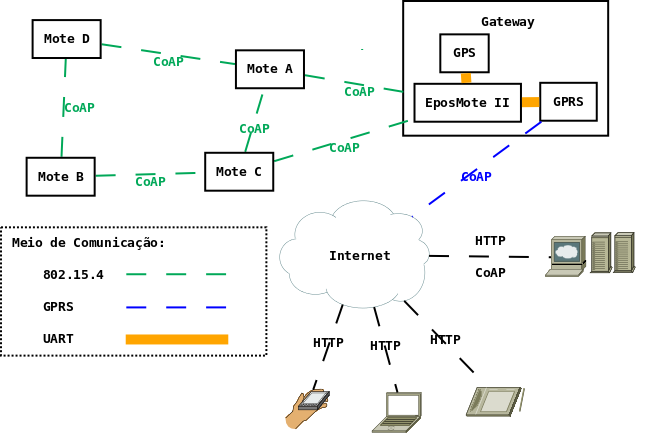
\includegraphics[width=0.8\textwidth]{figuras/arquitetura.png}
   \caption{Vis\~ao geral sobre comunica\c{c}\~ao do sistema.}
\end{figure}

\subsection{Componentes}
A aplica\c{c}\~ao do gateway \'e composta por: Mecanismos de temporiza\c{c}\~ao, camada UDP/IP, parser de pacote CoAP, conjunto de comandos AT, Estruturas de filas, Hash simples e Threads.

A implementa\c{c}\~ao consiste num m\'odulo que trata requisi\c{c}\~oes, encapsula em pacotes e transmite por mecanimos de transmiss\~ao baseados em \cite{draft-ietf-core-coap-18}.

A biblioteca utilizada para montar o pacote CoAP foi:\\https://github.com/staropram/cantcoap.git. Na qual enviei algumas corre\c{c}\~oes e testes para facilitar a verifica\c{c}\~ao da execu\c{c}\~ao correta dos algoritmos internos durante mudan\c{c}as no c\'odigo. As altera\c{c}\~oes podem ser visualisadas aqui:\\https://github.com/staropram/cantcoap/commits?author=rafaeldelucena.

Para o funcionamento desta biblioteca no EPOS, e para utilizar uma MTU limitada a 128 bytes utilizo um buffer com um valor m\'aximo e armazeno os dados do pacote no buffer. Foi necess\'ario alterar os tipos das vari\'aveis para se adquerem ao EPOS.

O desenvolvimento de um mecanismo de retransmiss\~ao de mensagens n\~ao-confirmadas utilizando uma lista ordenada. Mecanismo de requisic\c{c}\~o e resposta, as requisi\c{c}\~oes pendentes foram armezenadas num Hash com a chave sendo o token gerado pelo cliente.

O protocolo CoAP foi modelado conforme \'e mostrado na figura \ref{uml} abaixo:
\begin{figure}[h]
   \label{uml}
   \centering
   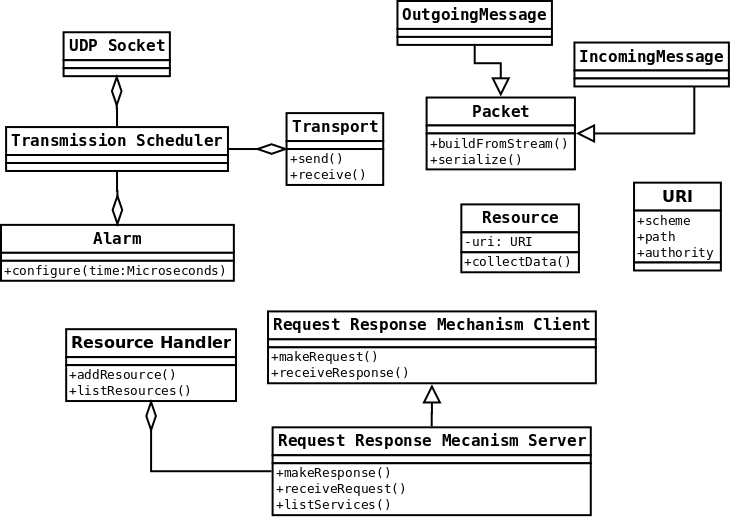
\includegraphics[width=0.9\textwidth]{figuras/uml.png}
   \caption{Diagrama UML das entidades de software implementadas.}
\end{figure}


\begin{figure}[h]
   \label{uml}
   \centering
   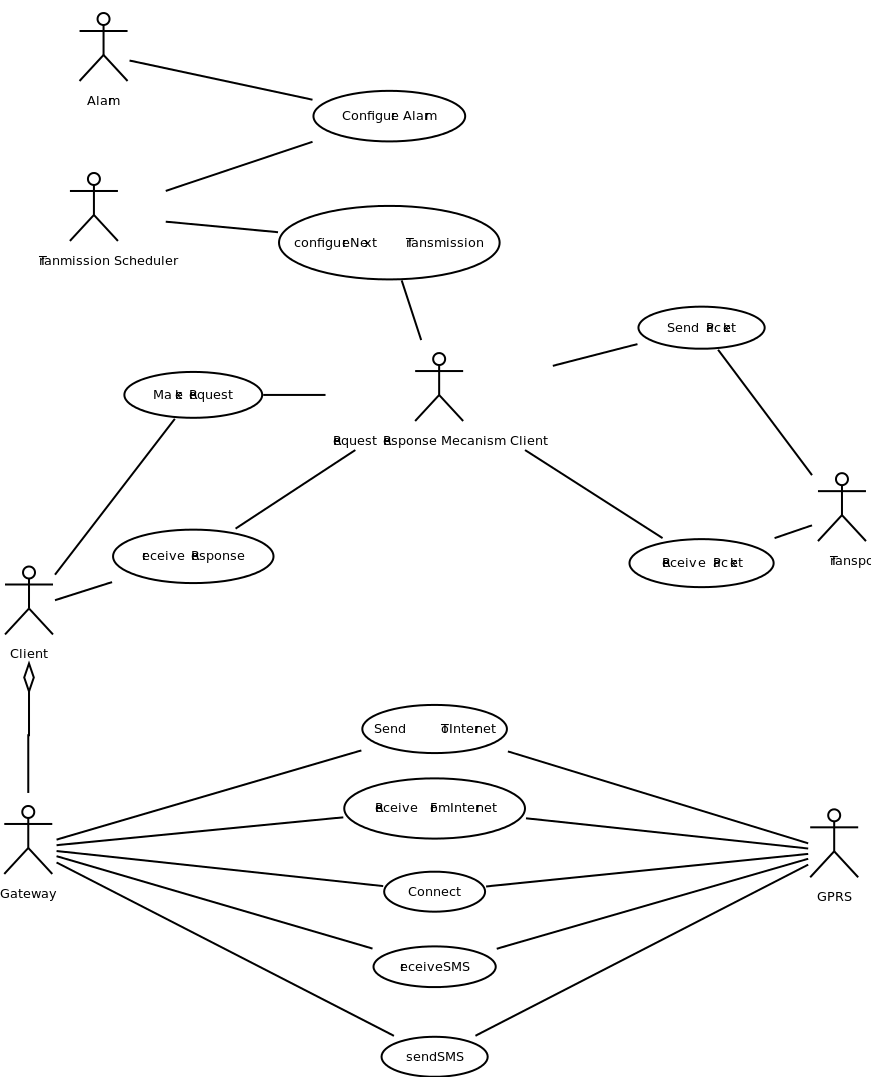
\includegraphics[width=0.8\textwidth]{figuras/casodeuso.png}
   \caption{Diagrama de casos de uso.}
\end{figure}

A aplica\c{c}\~ao cliente foi desenvolvida utilizando tecnologias HTML5. JavaScript, Json e HTML foram utilizados.
A biblioteca CoAP foi:\\https://github.com/mcollina/node-coap

A aplica\c{c}\~ao desenvolvida no EPOS utiliza buffer para o recebimento de dados da rede 802.15.4 que ser\'a enviado para rede via GPRS. Duas threads, uma produtora que ficar\'a escutando o r\'adio 802.15.4 e outra consumidora que ser\'a respons\'avel em utlizar estes dados na rede de sensores e encaminh\'a-los pra Internet usando a extens\~ao GPRS do EPOSmote II.

Para validar o comportamento utilizei alguns testes da pr\'opria biblioteca CoAP portados para o EPOS. Foi necess\'ario implementar a fun\c{c}\~ao assert. J\'a que seria bem mais trabalhoso adicionar uma ferramenta de testes no sistema de build do EPOS.

\section{Testes}

Foram realizados in\'umeros testes durante o desenvolvimento para verificar e validar o correto comportamento dos componentes de software e hardware.

Para validar a implementa\c{c}\~ao do protocolo CoAP foram efetuados os seguintes testes:
Testes de constru\c{c}\~ao de pacotes v\'alidos e inv\'alidos utilizando como entrada sequ\^encia de caracteres.
Testes de interoperabilidade entre as implementa\c{c}\~oes, utilizando cen\'arios parecidos com o IOT Plugtest.


Fazendo uma requisi\c{c}\~ao confirm\'aveis e n\~ao-confirm\'aveis do tipo: GET, POST, PUT, DELETE.
Recebendo respostas: válidas e inválidas.

Testes do Servidor:
Recebendo e respondendo requisi\c{c}\~oes: que possui recurso, que n\~ao possui, descoberta de recurso.

\subsection{Testes na placa de desenvolvimento do m\'ouldo GPRS}
Os testes feitos foram: Enviar e recebimento de mensagens; criar socket TCP, enviar e receber mensagem via socket, fazer requisi\c{c}\~ao HTTP, foi poss\'ivel utilizando os comandos propriet\'arios do modem.
